\chapter{Designing Exergames for Elderly}
\label{chap:exforseniors}

Exergames for elderly have become a popular topic in the past couple of years, and several research on how games can be developed for this particular user group have been conducted. Most of the research done on \ac{hci} are performed on young people \cite{dickinson2007methods}, and it is common to develop technology systems for a homogeneous user group. This means that the characteristics of specific user groups, like the elderly, are being ignored. With the wave of elderly ahead of us system designers have to put a greater focus on older people and their needs. Elderly in particular, have some special characteristics due to ageing that needs to be taken into account when developing technology systems for them. Studies indicate that most existing video games have not considered these characteristics, and are therefore not suitable for this group. 

In this chapter we will discuss elderly as users of a technology system. We will discuss characteristics of elderly that are important to acknowledge when designing technology systems for them. Based on previous research done on exergames for elderly people, we will draw out some specific guidelines that need to be considered when developing for this group. This can be found in Section \ref{sec:relatedresearch}. We will also provide previous research on elderly and user interfaces, as this is an important part of the gaming experience.  In addition, we will present some official guidelines for developing user-friendly interfaces for the elderly user. This will be provided in Section \ref{sec:designelderly}. 

\section{Related Research}
\label{sec:relatedresearch}
There have been done a lot of research on how to make exergames for seniors. In this section, we will review research that we have found to have interesting findings.

Billis et al. \cite{Billis} discuss important issues that need to be taken into account when developing games for elderly. Elderly often suffer from decline in visual acuity, decreased audition, mobility changes and cognitive functions' decline. In addition, many elderly are not familiar with technology. The writers suggest that it should be possible to customise the game for every player's special needs. Font, size and colour should be adjustable, and information should be provided in different multimedia alternatives, like text, voice and images. The objects should be of sufficient size and the elements should not move too fast. The overall interface should be as simple as possible, without the need to remember information given earlier in the gaming process, and it should be given sufficient information and guidance throughout the whole game. Games should also provide motivating messages to encourage the player. The writers also stress the importance of the social factors of the game, and suggest the ability to multi-play. At last, for the players to get interested and engaged in the game, they suggest that the content of the game should match the users' cultural and lifestyle diversity \cite{Billis}.

de Bruin et al. \cite{bruin} write about the potential of \ac{vr} environment, like exergames, for exercise. \ac{vr} platforms can evoke naturalistic movements in a safe environment that can be customised according to the patients' needs. It can offer a consistent program that enables for comparison over time. In addition, the use of games can distract the player from any pain they may have. They suggest stepping exercises to be suitable, because they have found that stepping exercises can be a good predictor of falls. It is also proved that a repetitive training program with stepping exercises can improve balance in elderly. Like they indicate in other research, \cite{gerling1} \cite{exergamesforelderly}, they also here express that the problem with already existing exergames is that they are too complex for the older user group. Therefore, there is a need to develop games specifically for this group where physical and cognitive limitations, as well as typical interests, are taken into consideration. The writers also present a study where it was shown a clear decrease in relative \ac{dtc} of walking for elderly. These elderly were training physically, combined with a virtual reality dance game that required decision making. Training traditionally, without the additional cognitive challenge, did not change these walking parameters. This comes from the fact that elderly people often face problems when they have to do more than one task at the same time \cite{bruin}.

Brox et al. \cite{exergamesforelderly} suggest some persuasive strategies for motivating elderly to exercise with games. They suggest that too much detailed information about the player's progress should be avoided. The information should rather be shown visually, like a fish that gets larger and healthier as the player is exercising. Information from previous sessions should be provided, to help players set new goals for the next session. The player should be provided with positive feedback as they achieve goals, and should not be punished if they do not achieve goals. This information and feedback should be given at an appropriate time, and should not disturb the player. The game should have an easy, understandable and good looking interface. The writers see social interaction as very important and suggest that this should be combined with exergaming. This is because it is shown that people get more engaged in activities when doing them with others, and because this group of people often suffer from loneliness and depression \cite{exergamesforelderly}. 

John et al. \cite{john2012smartsenior} write about the development of an interactive training system for seniors, called "Interactive Trainer". The main motivation for this system was the problem of falls. They refer to studies where it is shown that strengthening exercises, and balance and functional training, are suitable in the matter of reducing the risk of falls. They did a review of studies done on therapy for people over the age of 50, to find appropriate exercises to use in their training system. They found 12 concepts suitable for the "Interactive Trainer" system, where exercises for balance and strength were integrated. Their first exercises were (directly drawn from \cite{john2012smartsenior}: "walking while sitting", "weight shifting while sitting", "weight shifting to both sides while standing", "weight shifting to the front and rear while standing", "one-leg standing", and "sit-to-stand from chair".
      
The system consists of a computer and two motion sensor cameras. The movements tracked from these sensors are portrayed on a TV-screen or PC monitor. Ordinary internet connection makes it possible to communicate with the therapists through the system, both to get assistance and to transmit training results. The idea of "Interactive Trainer" is to provide individual therapeutic help to elderly, which they can benefit from in their own living room. They will be given a customised exercise program, and they will be provided with an evaluation of quality of the performed exercises. The seniors will be introduced for this game by therapists, where they together create a user profile, set up a training program, and choose avatar and preferred scenery. The seniors will then take the game home, where they will be guided by a virtual trainer. The exercises in the program have to be completed in a specific sequence, and a completion of one sequence of exercises will be rewarded with an "unlocking" of a new game. The therapist can follow the training from their "Interactive Trainer" editor, where they can supervise exercises, progress and success, and adjust the game accordingly. The writers acknowledge that success for the system is dependent on user acceptance, and essential for this is a good user interface and integration of motivational factors. To achieve this they use \cite{john2012smartsenior}:

\begin{itemize}
\item Avatar design in 3D
\item Virtual therapist in 3D
\item Motivational feedback systems, which will be used as encouragement  to reach goals
\item Corrective feedback systems, which will be used as guidance for exercise 
\item Tutorials for how to learn the system and chosen exercises
\item Target group-specific environment, with the use of familiar and real-life activities and exercises 
\end{itemize} 

Gregor et al. \cite{gregor} discuss some particular issues when designing for the older population. They propose a paradigm and methodology to support the process of designing software as close to the universal accessibility ideal as possible \cite{gregor}.

They describe older people through three different groups: Fit older people, frail older people and disabled people who grow older. In addition, they define some important characteristics of older people \cite{gregor}:
\begin{itemize}
\item As people get older the individual variability of physical, sensory and cognitive functionality will increase. 
\item Functional decline will go faster when people gets older. 
\item Cognition problems, like memory dysfunction and the ability to learn new things, are widely appearing.
\item Based on where they are in life, elderly may have different wants and needs. 
\item How people live, like if they are needing a walking frame or needing warm glows, can change their usability function.
\item Elderly have more life experience than younger people, and can therefore have more knowledge of the world, as well as a more mature ways of solving problems. 
\end{itemize}

To make it easier to develop a technology system for the older user group with different characteristics, Gregor et al. proposed a modified version of the \ac{ucd} principles, which they called \ac{usid}. The issues this methodology addresses are (directly drawn from \cite{gregor}): 
\begin{itemize}
\item "Much greater variety of user characteristics and functionality". 
\item "Finding and recruiting "representative users"". 
\item "Conflicts of interest between user groups (including "temporarily able-bodied")".
\item "The need to specify exactly the characteristics and functionality of the user group".
\item "Tailored, personalisable and adaptive interfaces".
\item "Provision for accessibility using additional components (hardware and software)".
\end{itemize}

As an example of the advantages of the proposed methodology, the writers present a case study where a web browser for people that are visually impaired was developed. 200 visually impaired users evaluated the system. The findings they did and the conclusions they made from this study were \cite{gregor}: 
\begin{itemize}
\item Elderly seemed to lack confidence in handling IT systems. However, the confidence increased after they had experienced a successful interaction and decreased after experiencing an unsuccessful interaction.
\item Many elderly had difficulties remembering too much information. This indicates that there are important memory related factors that need to be taken into account when designing for elderly. 
\item Following a need for less information, will most likely also mean less functionality. From another study they found that it was a need for the possibility that more functionality could be added after the user had mastered the initial, simple functionalities.
\item After some kind of assessment is passed, the user should be moved to a higher level. This can be done by self-assessment. To reinforce user-confidence the user should be able to reach goals. 
\end{itemize}

Gerling et al. \cite{gerling1} discuss possibilities and challenges when developing a game for elderly users, and they suggest four major guidelines to be followed:
\begin{itemize}
\item The player should have the possibility to interact with the game both when sitting and standing. 
\item Avoid too extensive and sudden movements.
\item It should be possible to adjust the level when it comes to difficulty, game speed and device sensitivity. These changes should be possible to be adjusted by the player. 
\item Interaction mechanisms should be simple, player frustration should be avoided, and the game should provide constructive feedback.
\end{itemize}

To verify these guidelines, the research group prototyped an exergame, called SilverBalance, made for the Wii Balance Board. SilverBalance consists of two balance tasks and has the possibility to be played both when sitting and standing. The game was tested on nine seniors with an average age of 84. The following observations were made \cite{gerling1}.
\begin{itemize}
\item All of the participants were able to play the game adequately. 
\item Participants expressed that the fact that the design was so minimalistic, made it possible for them to focus on the purpose of the game. 
\item The possibility to sit while playing the game was necessary because all participants were dependent on devices to assist them when standing and walking.
\item The players started to compare their results and comment on each other's results.
\item Impairments and diseases made it difficult for some participants after a longer period of playing, suggesting that alternative interactions should be included in such games.
\end{itemize}

The testing of SilverBalance shows that the four guidelines can contribute to the development of exergames for elderly people, but the writers state that further studies on how age-related changes can affect games, should be carried out \cite{gerling1}.

In another study, Gerling et al. present a case study where they introduce and evaluate an additional video game for elderly, called SilverPromenade \cite{gerling2}.  SilverPromenade is developed for the Nintendo Wii technology and utilises the Wii Remote and Wii Balance Board. The game is stripped from complexity in functionality and design to be senior-friendly. The theme of the game is a virtual "walk through the forest" and it can be played both as a single-player and multi-player game. In each mode of the game it is possible to engage three different roles: walking through the forest by stepping on the Wii Balance Board which requires physical exercise, catching a butterfly by pointing at it with the Wii Remote, and counting rabbits by shaking the Wii Remote when a rabbit appears. The scenarios are simplistic, which is important when including elderly in digital game play. The concept of the game was chosen because it appeals to elderly living in nursing-homes, as it offers them the possibility to "visit" the forest, which generally might be inaccessible for them. Playing this game requires the older player to focus on cognitive, mental and physical abilities. 

SilverPromenade has an easy and understandable user interface. Complex graphics and visual effects are avoided, while important elements are highlighted. It consists of a menu structure which easily guides the user to the playing-mode. The input devices used for playing makes it possible for elderly to both sit and stand during game-play, which takes the different individuals abilities into consideration.  If one of the three roles is not suitable, SilverPromenade offers the possibility of not including one or more roles.

A case study with SilverPromenade was executed on a group of frail elderly living in full-time nursing homes. The participants were asked to play the game and afterwards fill out a short questionnaire. Two groups of elderly participated, one group with experience with this type of technology, and one group without any experience. During the game play the researchers observed how the elderly used the controllers, how they understood the menu, and how easily they perceived the game behaviour. The gaming results were also observed.

Results from this case study show that experienced players clearly had an advantage over inexperienced players. It was observed during game play that some roles were difficult to execute, like when pointing at the butterflies they had difficulties using the Wii Remote because it required that one point it directly towards the sensor. However, the results showed that the overall experience was positive. SilverPromenade gave an impression of being outside, and the use of a real-world scenario engaged elderly to play. The concept of the game led to communication in terms of identifying objects, and helping and encouraging each other. One important observation was that the participants were sharing and discussing their scores. The conclusion of the case study was that elderly enjoyed playing digital games, and that SilverPromenade could be an appropriate game to use in this age group \cite{gerling2}.

Most studies done on elderly and the use of digital games, suggest that social interaction is important to include. Social interaction can be multi-play both in person in the same room and online. Online multi-play could be a good way to socialise for elderly who are less mobile and are lonely. However, not many studies on playing games together over the Internet have been conducted. We know that elderly often are unfamiliar with this type of technology \cite{Billis}, \cite{gregor}, and it is therefore important to acknowledge the challenges that can be faced by introducing multi-play over the Internet for this group. Gajadhar et al. \cite{Gajadhar} did a study, where they wanted to find out how players experiences playing together with different social presence. They tested a digital game on 40 participants in pairs with three different degrees of social presence: playing in the same room at the same time, playing against a computer controlled player, and playing together online. Results showed that while playing online elderly experienced low enjoyment, competence and challenge score, which indicates that they did not like playing online. It was also shown that they had more fun when playing alone, than when playing online with others. When playing together with others, they preferred seeing their co-players, and be able to speak with them. Seniors experienced more fun, competence, challenge and immersion when playing together in the same room than when playing with others over the internet. It was also found that seniors seemed to not care if they were winning or losing. They appeared to not be very competitive. Instead they enjoyed helping each other. The writers link this to previous studies that had found that elderly rather liked to help and teach others how to play games, than compete. The writers suggest that when including social interaction in games, the focus should be on cooperation rather than competition \cite{Gajadhar}. 


\section{Summary of Findings from Related Research}
\label{sec:summaryguidelines}
It is clear that elderly people have some specific characteristics that need to be considered when developing technology systems aimed for them. Based on the reviewed research we will summarise and list the discussed characteristics. In addition, we will draw out important aspects found in the literature, and list these as a proposal for guidelines to follow when designing an exergame for elderly.

\subsection{Characteristics of Elderly}
\label{subsec:characteristics}
\begin{enumerate}[{c}.1]
\item Cognitive functions' decline, e.g. dementia, memory dysfunction, and the ability to learn new things \cite{Billis}, \cite{gregor}.
\item Decline in sensory functionality, like  visual acuity and audition \cite{Billis}, \cite{gregor}.
\item The problems elderly face, often increase significantly with increasing age \cite{gregor}.
\item Mobility change \cite{Billis}.
\item Needs and wants related to cultural and lifestyle diversity, as well as at what stage they are in life \cite{Billis}, \cite{gregor}.
\item Many are in need of assistant tools (for example when standing and walking) \cite{gregor}.
\item Inexperienced with technology. Many elderly people seem to lack confidence when it comes to IT-systems. A better confidence can be achieved when experiencing a successful interaction with an IT-system \cite{Billis}, \cite{gregor}.
\item It is important to take into account memory related factors. Many elderly have difficulties remembering too much information \cite{Billis}, \cite{gregor}.
\item It can be challenging to do more than one task at the same time \cite{bruin}.
\end{enumerate}

\subsection{Proposed Guidelines from Related Research}
\label{subsec:guidelines}

\begin{enumerate}[{g}.1]
\renewcommand{\labelitemi}{$\bullet$}
\item The game should have the possibility to be customised for every user's needs, conditions, interests etc. \cite{Billis}, \cite{bruin}, \cite{gregor}, \cite{gerling1}, \cite{john2012smartsenior}.
\item The interface should offer adjustable font, size and colours \cite{Billis}.
\item The interface should have different alternatives for multimedia presentation, for example, text, voice and images \cite{Billis}.
\item The interface should be simple and not too extensive. The objects should be of sufficient size and there should be no sudden movements. Important elements should be highlighted \cite{exergamesforelderly}, \cite{Billis}, \cite{gerling1}, \cite{gerling2}.
\item The game should have a menu, which easily guides the user to the gaming session \cite{gerling2}, \cite{john2012smartsenior}.
\item Sufficient guidance and information should be given before and during the process. There should not be a need to remember earlier given information \cite{Billis}, \cite{gregor}, \cite{john2012smartsenior}.
\item Motivating feedback should be given to encourage play \cite{Billis}, \cite{gerling1}, \cite{exergamesforelderly}, \cite{john2012smartsenior}.
\item Constructive feedback should be given to guide and correct exercises \cite{john2012smartsenior}. 
\item Information and feedback should be given when appropriate, to not disturb the player \cite{exergamesforelderly}.
\item The story of the game should match cultural and lifestyle diversity \cite{Billis}, \cite{gregor}, \cite{gerling2}. 
\item The game should use environments and activities that are familiar to the target group. An example presented in \cite{gerling2} is a game with a real-world scenario, where the players have to walk through a forest. \cite{john2012smartsenior}, \cite{gerling2}.
\item Social factors should be included by offering the possibility to multi-play \cite{Billis}, \cite{gerling2}, \cite{gerling1}, \cite{exergamesforelderly}.
\item Multi-play should focus more on cooperation than competition \cite{Gajadhar}.
\item It should be offered variety in user characteristics and functionality \cite{gregor}, \cite{gerling1}.
\item The game, with its environment and characters, should be in 3D to enhance the gaming experience \cite{john2012smartsenior}.
\item The game should not have too much functionality, but instead offer the possibility to add more functionality after the existing functionalities are managed \cite{gregor}, \cite{gerling2}.
\item The game should offer different levels with different difficulties. With this comes the possibility to reach goals. The device sensitivity and the game speed should also be adjustable \cite{gregor}, \cite{gerling1}, \cite{john2012smartsenior}.
\item The game should give the player information about progression and results. This information should not be too extensive \cite{exergamesforelderly}, \cite{john2012smartsenior}.
\item It should be possible for the player to adjust levels themselves \cite{gregor}, \cite{gerling1}. 
\item The possibility to interact with the game both when sitting and standing is important \cite{gerling1}, \cite{gerling2}.
\item The game should use exercises which are proven to be good for elderly \cite{john2012smartsenior}. 
\item Exergames for elderly should have the opportunity to be used in a clinical setting \cite{Billis}, \cite{gerling2}, \cite{john2012smartsenior}.
\item There should be made a profile where the user's progress and results can be saved. If the game is used in a clinical setting, it should be possible to share this profile with therapists \cite{john2012smartsenior}. 

As an additional guideline, it is worth mentioning that both \cite{bruin} and \cite{gerling2} discuss stepping as a relevant exercise for elderly. This is because this kind of exercise has proved to be a good predictor of fall and that repetitive stepping exercises can improve balance. Stepping requires significant physical activity, which is important when improving physical health. Walking or stepping exercises are also recommended by the Department of Health and Human Services, discussed in Chapter \ref{chap:olderexercise}. In addition, \cite{john2012smartsenior} mentions balance and functional training, together with strengthening exercises, as appropriate for elderly as it can lead to reducing the risk of falling.    

\section{Guidelines from Official Organisations for How to Design User-Friendly Interfaces for Elderly}
\label{sec:designelderly}

As seen from the characteristics in the previous section, ageing will often lead to both physical and psychological negative changes, like decline in cognitive skills, visual and auditory acuity, and in balance and physical strength. An important part of game development is designing the user interface, where having an intuitive and user-friendly interface is crucial for the game to experience acceptance and success.  When working on interface design, the users' needs have to be taken into consideration, and designers should therefore take into account the characteristics of elderly when developing a game for this user group \cite{mmi}. Especially, when designing an interface for elderly, the aspect of visual decline is important to focus on \cite{blindeforbundetTekst}. 

There exist various examples of guidelines for how to design good and user-friendly interfaces for elderly, or people in general, that are partially sighted or visually impaired. Visual decline implies less contrast sensitivity, decrease in peripheral vision, and more dark adoption \cite{ijsselsteijn2007digital}. Therefore, some of the main guidelines are simple design, large font size, and sharp contrast between background colour and font colour. The users might have different levels of visual decline, so it is preferable to allow users to change settings themselves \cite{blindeforbundetTekst} \cite{actionforblindpeopleTekst} \cite{w3cTekst}. Design guidelines are provided by various organisations, as e.g. "Blindeforbundet", a Norwegian federation for everyone with poor vision \cite{blindeforbundet}, "Action for Blind People", a charity in the UK which provides support to people that are blind or partially sighted \cite{actionforblindpeople}, and "World Wide Web Consortium (W3C)", a community working together to create web standards \cite{w3c}. These web standards are meant to be used as guidelines for making usable interfaces for the general user, regardless of age or disabilities \cite{w3cTekst}. These three organisations are just a few out of several others with focus on making technology accessible for elderly and people with visual disabilities. 

We will now present a summary of guidelines to consider when designing an interface for elderly, gathered from the three organisations mentioned above. The numbering of the guidelines will continue from the numbers presented in the previous section as all these will be used together as guidelines when developing the exergame.


\textbf{Make the text easy to read} \\ \\

\item Use a relatively large font size, minimum 12 pt \cite{blindeforbundetTekst}. A font size of 14-16 pt is preferable for those who are visually impaired. For large prints 16-22 pt should be used \cite{actionforblindpeopleTekst}. Use of font size larger than 20 pt will not increase readability in a text \cite{blindeforbundetTekst}.     
\item Use a clear print. This mean that a sans serif font should be used (see Table \ref{tab:fonts}). Arial, Helvetica and Futura are fonts that are easy to read \cite{actionforblindpeopleTekst}.

\begin{table}
\centering
\begin{tabular}{ l p{8cm} }

\multirow{1}{*}{
\includegraphics[scale=0.6]{font1.jpg}} & This is the letter X in Times New Roman, a widely used font. The lines have various widths, and there is a broader design at the ends. \\ \\ \\ \\
\multirow{1}{*}{
\includegraphics[scale=0.6]{font2.jpg}} & This is the same letter in Arial. This font is easier to read for those with visual decline. Here the lines are equally wide all over, without the expansion at the ends. \\ \\

\end{tabular}
\caption[Fonts]{Fonts with and without serifs [modified from \cite{blindeforbundetTekst}]}
\label{tab:fonts}
\end{table}
\item Avoid fonts with special styles \cite{blindeforbundetTekst} \cite{actionforblindpeopleTekst}.
\item For titles, use upper-case letters in beginning of words \cite{actionforblindpeopleTekst}. Do not use capital letters in large amounts. They give little variation, which makes the text difficult to read \cite{blindeforbundetTekst}. 
\item Do not use italics, underlining and bold typing in a larger coherent text, that will disturb the reading \cite{blindeforbundetTekst} \cite{actionforblindpeopleTekst}.  
\item If possible, allow the users to change font and text settings themselves \cite{blindeforbundetTekst} \cite{w3cTekst}. 
\item Use a language with ordinary, well-known words. This makes the text more easy to understand \cite{w3cTekst}. \\ 


\textbf{Use simple design}

\item Use simple design, as this makes it easy for important elements to stand out \cite{actionforblindpeopleTekst}.
\item Be consistent in design and layout throughout the system \cite{actionforblindpeopleTekst}.
\item Always use left-aligned text. Centered text appears unclear \cite{actionforblindpeopleTekst}.  
\item Keep spacing between words permanent. Do not stretch the text to get an even right margin, as this will change the spacing randomly. An uneven right margin is good for readability, as it help leading the eyes to the next line \cite{blindeforbundetTekst} \cite{actionforblindpeopleTekst}.
\item Do not use too much or too little spacing between lines \cite{blindeforbundetTekst} \cite{actionforblindpeopleTekst}. 
\item Avoid big blocks of text. The text will be easier to read and understand if it is divided into smaller sections \cite{blindeforbundetTekst} \cite{actionforblindpeopleTekst}. \\  


\textbf{Use of colours and contrasts}
\item It is important with sharp and clear contrast between background colour and font colour to ensure good readability \cite{blindeforbundetTekst} \cite{actionforblindpeopleTekst}. The actual choice of colours is not that essential.   
\item In general, the most preferred combination of background colour and font colour is black text on either white or yellow background \cite{actionforblindpeopleTekst}. Black on white or yellow creates a very good contrast \cite{blindeforbundetTekst}. 
\item People are different. Some might prefer the opposite, like light font colours on dark background \cite{blindeforbundetTekst}. This again suggests that it should be possible to customise settings. When using light font colours on dark background, the font should be both bigger and bolder to make the text more readable \cite{actionforblindpeopleTekst}.
\item Avoid pale colours on coloured background \cite{blindeforbundetTekst}.  
\item Choose a one-coloured background. Try not to write text on pictures. The picture will take the attention away from the text, and make the text harder to read. If necessary, put the text where there is light areas in the picture  \cite{blindeforbundetTekst}.  
\item Reading speed is also highly connected to colours and contrast  \cite{blindeforbundetTekst}. Black text on white background provides the highest reading speed in a text. For more combinations, see Figure \ref{fig:contrastreadingspeed}.

\begin{figure} [ht!]
\centering
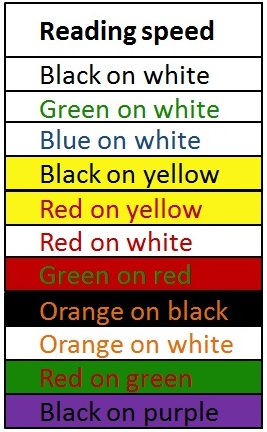
\includegraphics[scale=0.5]{readingcolors.jpg}
\caption[Colours and contrasts - reading speed]{Relationship between choice of text and background colour, and reading speed. The best combinations are those shown on top. (Translated from Norwegian, \cite{blindeforbundetTekst})}
\label{fig:contrastreadingspeed}
\end{figure}

\item By choosing text and background colour according to the surrounding environment, readability can be increased \cite{blindeforbundetTekst}. Table \ref{tab:contrastenvironment} shows appropriate colour combinations for four environments. These combinations are meant for digital information boards out in the real world. The choice of colours will also make the board stand out from its environment.  

\begin{table} [ht!]
\centering
    \begin{tabular}{|p{3,8cm}|p{2,3cm}|p{4,9cm}|}
       \hline
       \textbf{Environment} & \textbf{Background} & \textbf{Text} \\ \hline
		Red brick, dark stone & White & Black, dark green, dark blue \\ \hline
		Light brick, light stone & Black, dark & White, yellow \\ \hline
		Whitewashed wall & Black, dark & White, yellow \\ \hline
		Green vegetation & White & Black, dark green, dark blue \\ \hline
    \end{tabular}
    \caption[Colours and contrasts - environment]{This figure shows how text and background colour should be chosen according to the environment to ensure good readability. (Translated from Norwegian, \cite{blindeforbundetTekst})}
    \label{tab:contrastenvironment}
\end{table} 


\textbf{Provide accessible information}
\item Provide alternatives for how to present information. For those who are visually impaired, an audio presentation might be preferable \cite{blindeforbundetTekst} \cite{w3cTekst}. 
\item Text is a better way to present information than use of images and icons \cite{w3cTekst}.
\item Give the users time to read the given information. Let them tell the system when they are finished reading \cite{w3cTekst}.  
\item Help users to easily navigate to the content of interest \cite{w3cTekst}.
\item Assist users on how to avoid and correct mistakes. Describe the error for the user, and provide a suggestion for how they can undo the action that caused the error \cite{w3cTekst}.      
\end{enumerate} 

The characteristics and guidelines drawn from previous studies together with the official guidelines proposed by "Blindeforbundet", "Action for Blind People" and "World Wide Web Consortium (W3C) will become very important  when we develop a concept for an exergame for elderly. To understand how to design this exergame, we also have to understand how video games in general can be designed. This will be described in the next chapter.




